\section{Diagnostics}
%\todo{Use \textbackslash SI \{\}\{\} for the units}
% In your teams, please write a short \textit{Executive Summary} with a \textbf{\textcolor{red}{maximum of 3}} pages.\\
% Please include the following headers in your summary, and try to talk about some of the following tasks and questions, but feel free to adapt the guideline to your needs and liking. Everyone's welcome and encouraged to edit this document! (\textit{not} just the speakers)\\

% \textbf{\textcolor{red}{Deadline 10.07.2024}}\\

% \textit{At first, please introduce your Team and why it's needed for designing a fusion reactor}

Diagnostics are needed to validate the calculated magnetic field as well as measure the densities and currents. For this, the diagnostics team designed an interferometer, a 2D-manipulator for the Langmuir probe in the y-z-direction, with a changeable probe tip, a fluorescence rod, a concept for
a Rogowski coil measurement, concept for a diamagnetic coil measurement and a price comparison for different types of lock-in amplifier for a low temperature stellarator which has a configuration of $B=87~\unit{mT}$, $n_e < 10^{18}~\unit{m^{-3}}$ and $T_e=10~\unit{eV}$.
% With these we can measure...


\subsection{Requirements and Tasks}

% \textit{What are the requirements your system has to fulfill to build the small reactor? What do other teams require from you? What are the topics you first had to investigate on? Please include your tasks, what you did as a Team during the semester. What did you look into? What implementations did you consider (but maybe rejected later)?}\\

The interferometer measures the change in phase of a wave due to the plasma and relates it with the line integrated electron density of the plasma. First the maximum magnetic field and density need to be known, see above, to determine the maximum electron cyclotron and electron plasma frequency. Then it was shown that when a wave is sent into a magnetized plasma in such a way that the direction of propagation is perpendicular to the magnetic field, the ordinary wave, which has an oscillating electric field parallel to the magnetic field has a an index of refraction of $N = \sqrt{1 - \frac{\omega_\mathrm{pe}^2}{\omega^2 }}$. This means that the wave needs to be sent in at a right angle to the magnetic field and with a frequency higher than the electron plasma frequency, which for our values is $9$ GHz. When writing the resulting phase shift as a function of the frequency, the simplification that $\omega \gg \omega_\mathrm{pe}$ was used, meaning a frequency $f \gg$ 9 GHz. Using Gaussian beams it was possible to derive the optimal dimensions of the mirror reflecting the wave. It is based on the frequency used and the distance between horn antenna and mirror which depends on the plasma diameter. Depending on the geometry of the vacuum vessel the horn antenna, which sends the wave, as well as the horn antenna that receives the reflected wave, can be placed inside the vacuum chamber. For this the geometry and the space available inside the chamber need to be known to calculate the positions of the horn antenna as well as the reflecting mirror. \\

The magnetic diagnostics has to extract the plasma currents out of a large background noise. In this project, the magnetic diagnostics consists of two diamagnetic coils, one Rogowski coil, and signal processing equipment. 
The diamagnetic coils measure the poloidal plasma current. 
The Rogowski coil measures the toroidal plasma current. 
The signal processing
equipment consists of several lock-in amplifiers, low- and band-passes and D/A converters. They filter out the background noise, and amplify the plasma current signals. \\

For the Langmuir probe it is needed to scan the cross-section of the plasma to measure the $I-V$-characteristic of the plasma. With this characteristic plasma parameters are fitted (the floating potential $\Phi_\mathrm{fl}$, the plasma potential $\Phi_\mathrm{p}$, the electron current $I_\mathrm{e}$, the ion current $I_\mathrm{i}$, the electron saturation current $I_\mathrm{e,sat}$, the ion saturation current $I_\mathrm{i,sat}$ and the electron plasma density $n_\mathrm{e}$).

In the left image of Figure~\ref{fig:probe characteristics and CAD_Interferometer and CAD_changeable_probe_tip} we can see that the electron saturation current has different curve shapes for different probe tips, for example for a spherical, cylindrical or a flat tip. The flat tip has the \emph{sharpest} bend of all the tip geometries.
The floating potential is the root of the $I-V$-characteristic, which occurs when the ion current and electron current are equal, negating each other resulting in zero current.
The saturation currents exists because when the probe is charged one way, for example positive, all electrons in a region around the probe fly towards the probe. However, due to Debye shielding the created depletion region cannot grow indefinitely. Once it reaches its maximum the current saturates and only thermal electrons outside the region enter the probe. The corresponding voltages are the plasma potential and the floating potential. With following equation the current of the probe can be determined:

\begin{equation}
    I=I_i+I_e=enS \sqrt{\frac{T_e}{2 \pi m_e}}
    \Biggr[0.61 \sqrt{\frac{2 \pi m_e}{m_i}}-\exp\Bigl\{-\frac{e(\Phi_p -U)}{T_e}\Bigr\}
        \Biggl]
\end{equation}


\begin{equation}
    I^*_{e,sat} =I_{e,sat}\Biggr[1+ \frac{e(U-\Phi_p)}{T_e}\Biggl]^{\gamma_{om}}
\end{equation}
where $\gamma_{om}= 1/2$ is for cylindrical probe tips and $\gamma_{om}= 1$ is for spherical probe tips. \cite{Stroth_Plasmaphysik}



\subsection{Outcome}

%\textit{What's the outcome of your study? What does your design look like in the end? What did you decide on and why? Maybe include some parameters, please include finalized designs \& CAD models}
Having evaluated the basic parameters for the interferometer the schematic of the circuit was designed. The difficulty lies in measuring a phase shift occurring at a GHz frequency. For this purpose mixing the signals with a  Gunn diode ring modulator is used to function as a downconverter. The local oscillator (LO) is run with a frequency $\omega$ and the reference oscillator (RO) with the frequency $\omega + \Delta \omega$, see the right image of Figure~\ref{fig:2D-manipulator and probe tip and interferometer_circuit_schematic}. With two mixers and amplifiers and band-pass filters we manage to get a signal with the frequency $\Delta \omega$. When we use a $\Delta \omega$ in the MHz range we can detect the phase shift with a phase detector. If there is not enough space inside the vacuum space an alternative design with Teflon lenses was also explored, see~\cite{2012JInst...7C1107C}. A python script was written with which one can calculate the ideal distances for every geometry and frequency. \\

Reagrding the Rogowski coil, the basic principles of the coil were explored. The
diamagnetic effect in linear pinches was shortly reviewed, and different options regarding the lock-in amplifiers were examined.
Simple CAD-models of the Rogowski and diamagnetic coils were created.

\begin{figure}[h]
    \centering
    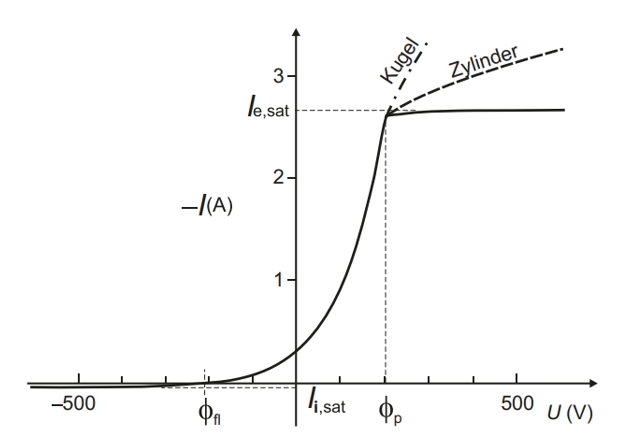
\includegraphics[width=0.3\linewidth]{Images/04_Diagnostics/probe characteristic.png}
    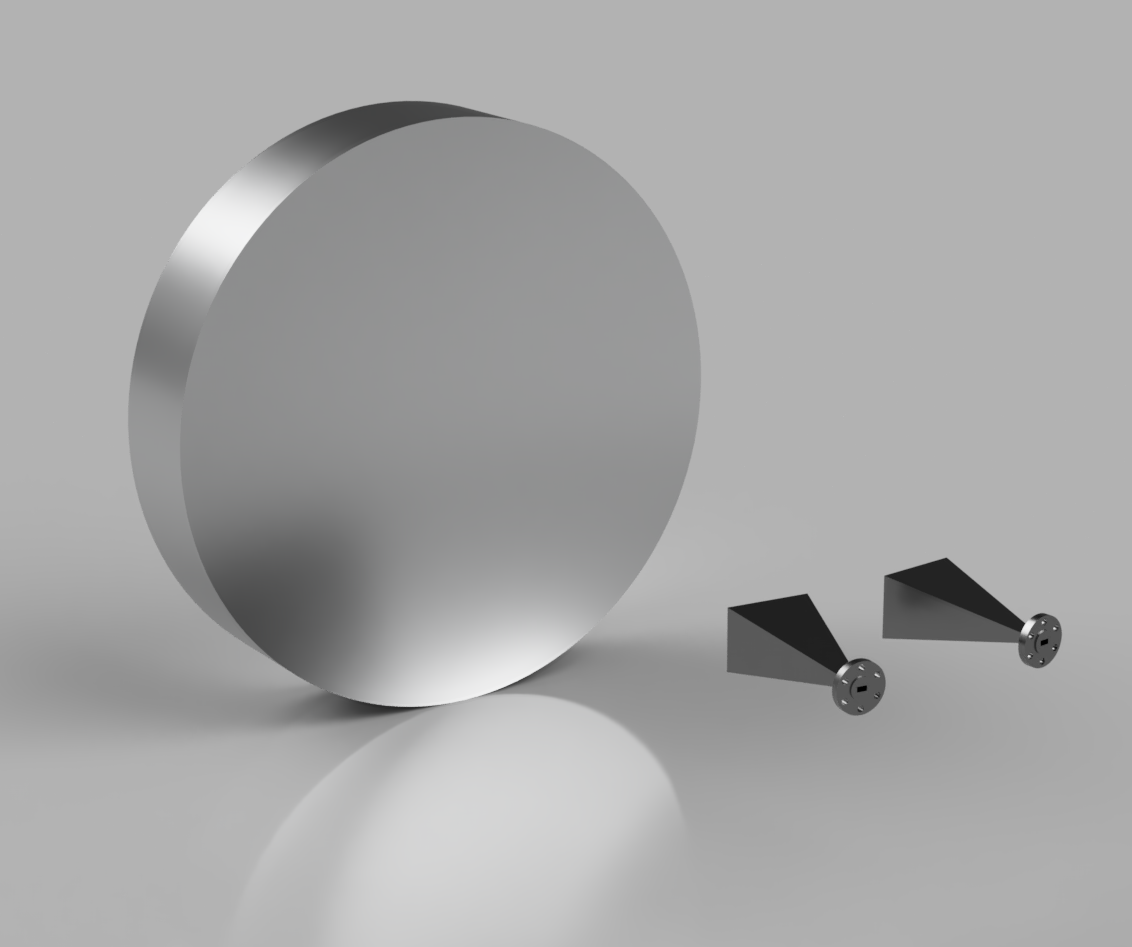
\includegraphics[width=0.3\linewidth]{Images/04_Diagnostics/CAD_Interferometer.png}
    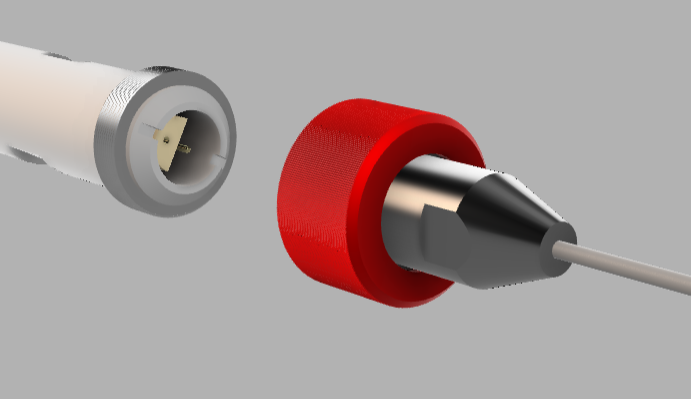
\includegraphics[width=0.3\linewidth]{Images/04_Diagnostics/CAD_changeable_probe_tip.png}
    \caption{Left: I-V-characteristic of a Langmuir probe \cite{Stroth_Plasmaphysik}. Middle: plasma CAD of the interferometer for a certain frequency and distance. Right: 3D-model of the changeable probe tip with a union nut.}
    \label{fig:probe characteristics and CAD_Interferometer and CAD_changeable_probe_tip}
\end{figure}


The outcome at the Langmuir measurement was the geometry of the Langmuir probe tip which has a radius of $0.125$~mm, a probe tip made out of tungsten, an isolation layer of aluminum oxide with the dimension of outer diameter of $1$~mm and a inner diameter of $0.5$~mm, a designing concept of a  2D-manipulator for the Langmuir measurement and the design of a changeable probe tip. Also the position and the geometry for the flange (DN400 ISO-F) at the vacuum vessel was determined. Additionally, a design of the small vacuum chamber for the manipulator was created. It includes a power feed-through, a ball valve, a UHV slider to get a closed chamber for maintenance. Inside of the chamber there is a sliding system in three dimension to get a $z-y$-movement for the probe. The slinding bearings are made of iglidur\textsuperscript{\tiny\textregistered}, because the use of any type of lubricant in the vacuum area is not recommended and this material absorbs little moisture. The left image of Figure~\ref{fig:2D-manipulator and probe tip and interferometer_circuit_schematic} shows the 3D-model of the 2D-manipulator and the changeable probe tip.




\begin{figure}[h]
    %\centering
    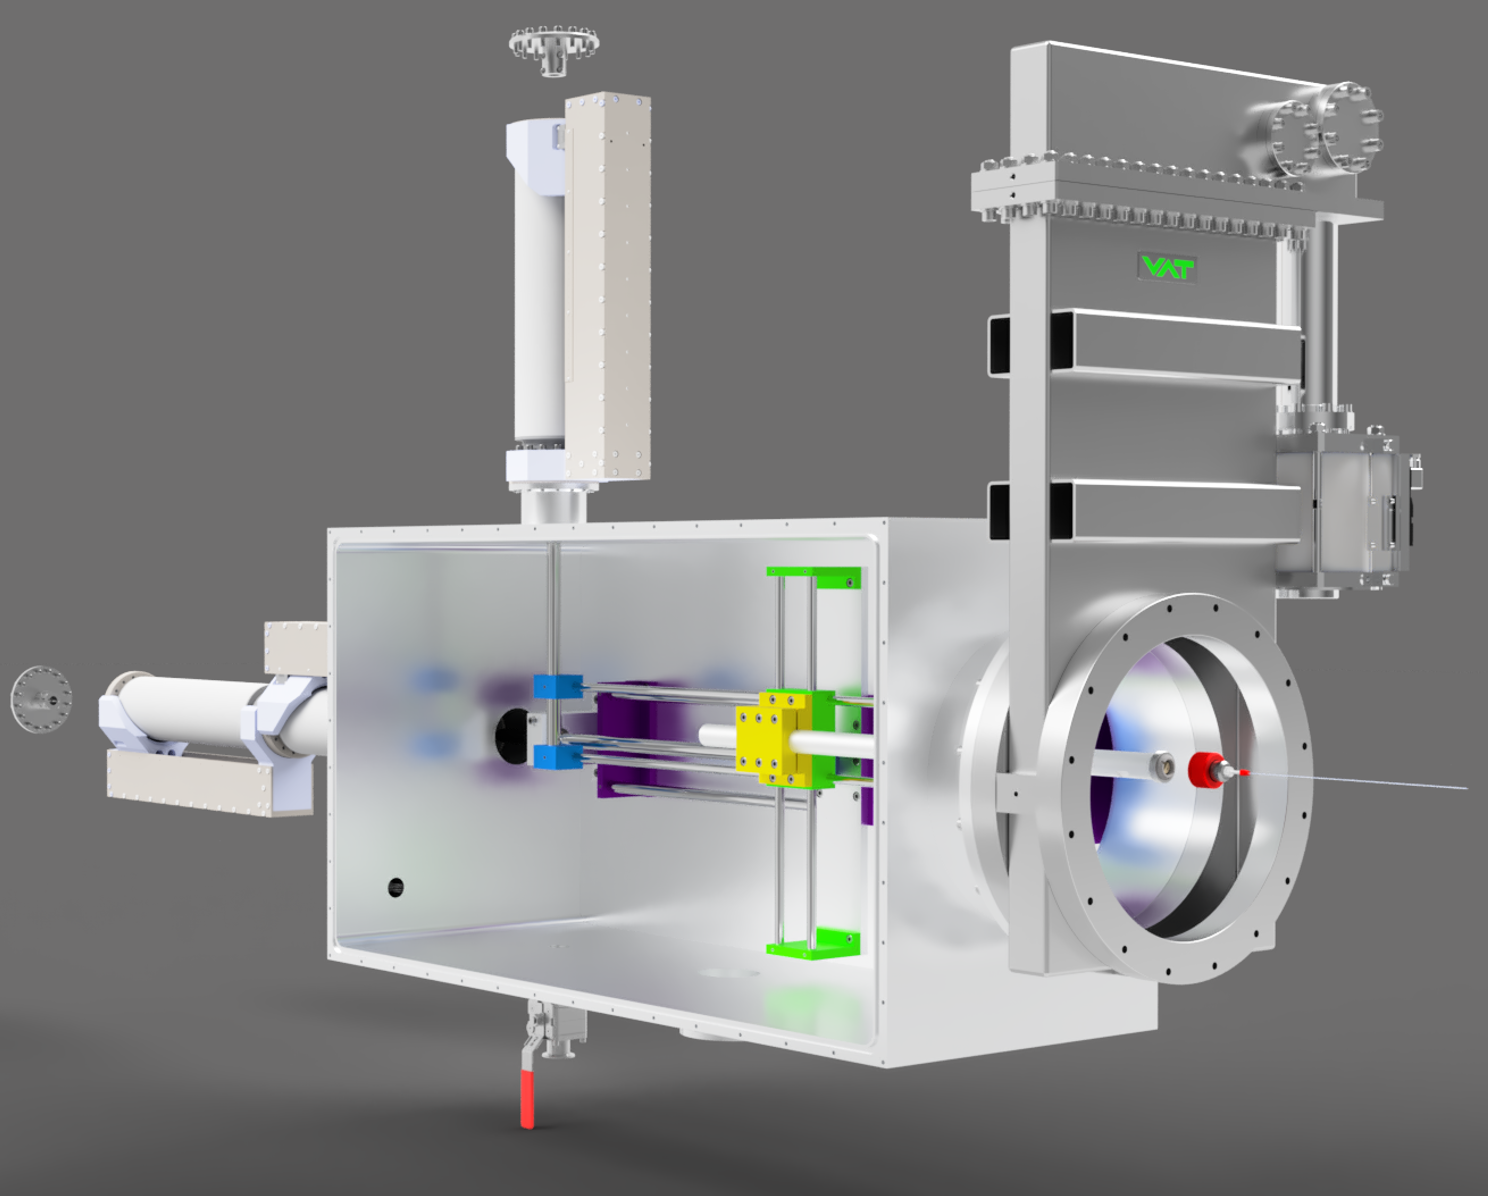
\includegraphics[width=0.4\linewidth]{Images/04_Diagnostics/CAD_2D_manipulator.png}
    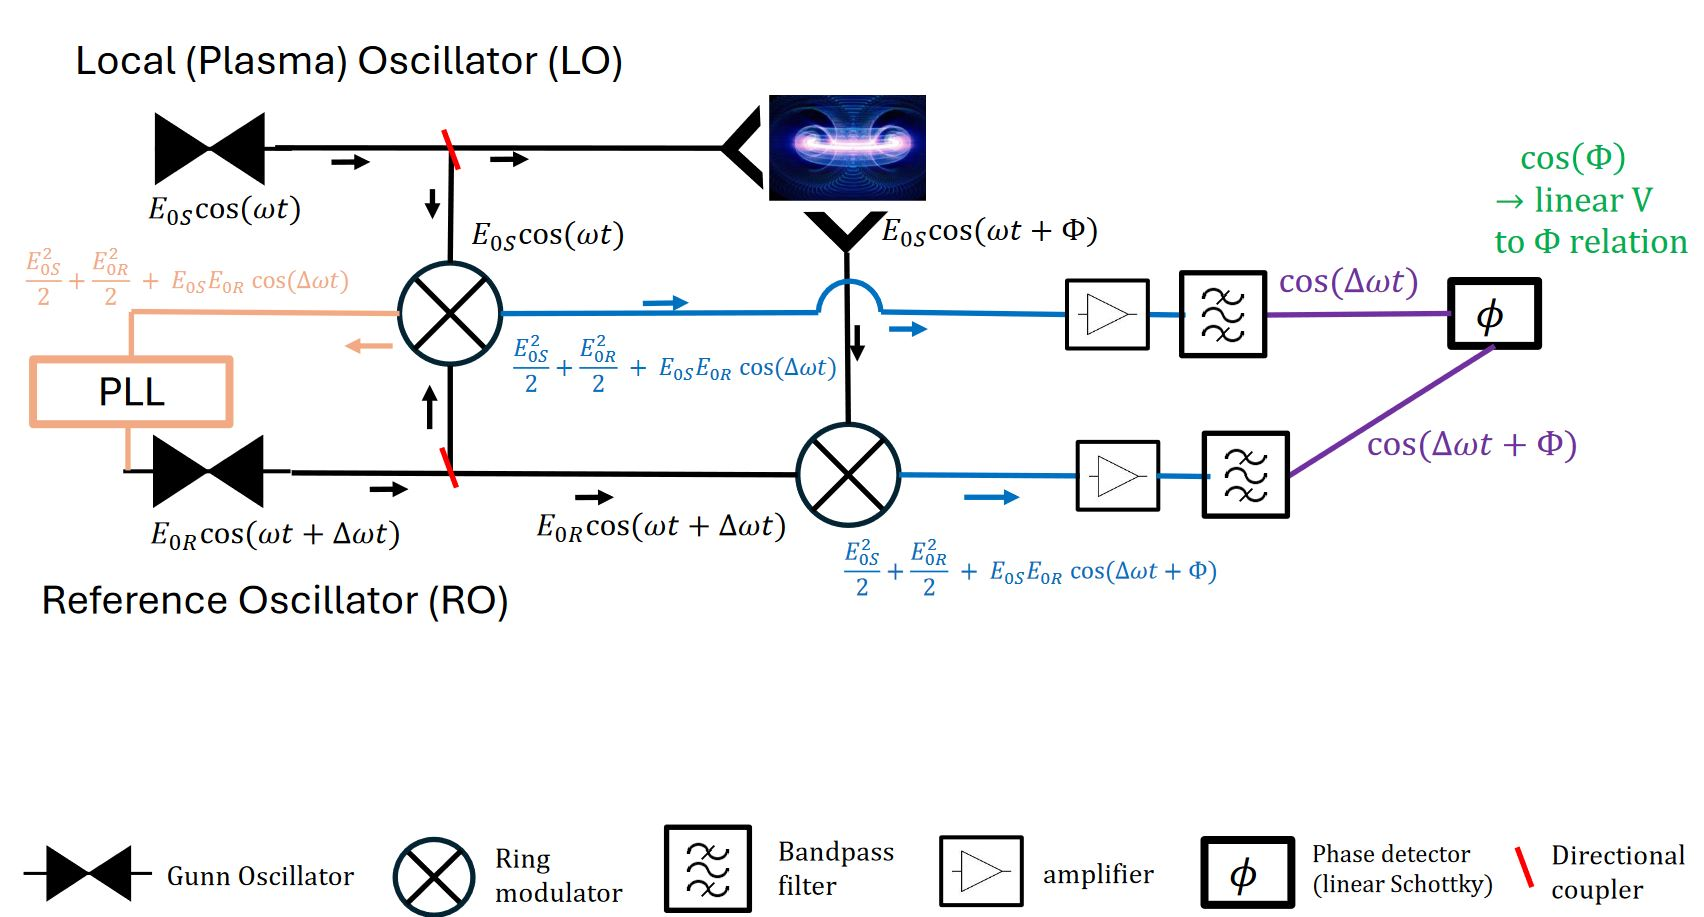
\includegraphics[width=0.59\linewidth]{Images/04_Diagnostics/interferometer_circuit_schematic.JPG}
    \caption{Left: 3D-model of the 2D-manipulator with a Langmuir probe.  Right: Schematic of the circuit of the interferometer.}
    \label{fig:2D-manipulator and probe tip and interferometer_circuit_schematic}
\end{figure}



The outcome at the measurement of the magnetic flux lines was to design a fluorescence rod which has a coating of zinc-oxide (ZnO:Zn). The design for the rod was implemented to the changeable probe holder which has the same plug. Also an electron gun was designed.


\subsection{Outlook}

%\textit{Where could a future team continue your work?}

Gather together with electric/electronic staff  of other teams to
centralize power supply/signal processing.
Further explicate requirements for signal processing equipment.
Refine the preliminary
CAD models of the Rogowski and diamagnetic coil.
After deciding an oscillator with a certain frequency once can fix the geometry of the mirror and work on the mounting of the mirror. Similarly the circuit can be refined and the powers and voltages can be calculated. Finally, the appropriate hardware can be looked into and acquired.
The observation window can be used for passive spectroscopy and additional diagnostics tools could also be designed to compliment the current instruments. It is necessary to choose the right material and a possible wall thickness for the vacuum chamber of the 2D-manipulator and the dimension. To design a 1000~mm manipulator for the 2D-manipulator on the side. The evaluation of the measurement and implement to LabVIEW. Designing an electron gun.


\subsection{Learnings}

%\textit{What did you learn during this coursework? What are some problems you encountered? What roadblocks did you hit?}

Some basic properties of a static plasma configurations were learned.
Concepts behind the lock-in technique were reviewed.
Great difficulties were encountered in using the Autodesk Fusion CAD software.
In order to understand the interferometer we learned plasma wave physics as well as the propagation of a wave in a waveguide and in the horn antenna. Furthermore we learned about signal processing, however we did not have much experience in that regard so we are still not sure if we chose the ideal circuit or if there are complications we have not thought of. A new 3D-CAD software and implement movements in the assembly group. Design movement parts in vacuum and use the right bearings. Design layout of different plasma measurement systems. Concepts behind the Langmuir probe measurement and the measuring of a closed magnetic flux field. Cross-team collaboration.
